\section{Phụ lục}

\begin{figure}[H]
    \centering
    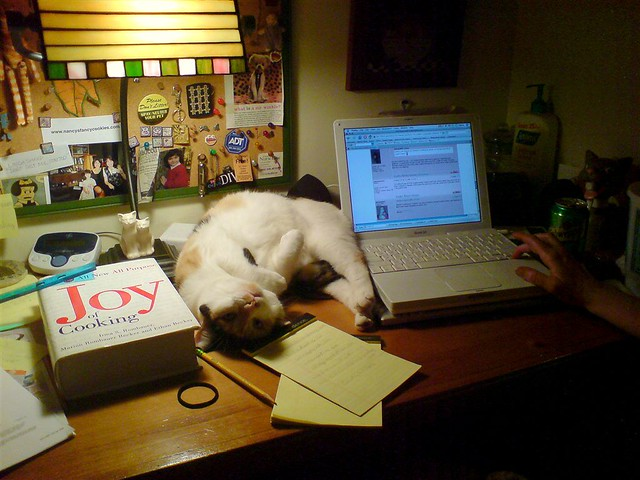
\includegraphics[width=0.75\linewidth]{appendix/cat-image.png}
    \caption{Hình ảnh một con mèo nằm giữa một cuốn sách và một cái laptop, trên một cái bàn nhỏ.}
\end{figure}


\begin{table}[H]
\centering
\begin{tabular}{|l|l|l|}
\hline
Văn bản cho trước           & \textbf{CLIP} & \textbf{ALIGN} \\ \hline
'a photo of a cat' & 0.0228        & 0.0018         \\ \hline
'a photo of a dog'          & 0.0020        & 0.0000         \\ \hline
\begin{tabular}[c]{@{}l@{}}'cat lying between \\ laptop computer and \\ book on small desk'\end{tabular} & 0.9752 & 0.9982 \\ \hline
\end{tabular}
\caption{Kết quả so sánh độ tương đồng ảnh-văn bản bởi CLIP và ALIGN}
\label{tab:CLIP-ALIGN}
\end{table}

\begin{table}[H]
\centering
\begin{tabular}{|l|l|}
\hline
Tác vụ                                                                    & \textbf{BLIP} \\ \hline
\begin{tabular}[c]{@{}l@{}}Tạo chú thích ảnh \\ (Image Captioning)\end{tabular} & \begin{tabular}[c]{@{}l@{}}a cat is sleeping on a \\ desk with a laptop\end{tabular} \\ \hline
\begin{tabular}[c]{@{}l@{}}How many cats are there? \\ (VQA)\end{tabular} & 1             \\ \hline
\begin{tabular}[c]{@{}l@{}}What is the cat's color?\\ (VQA)\end{tabular}  & white         \\ \hline
\end{tabular}
\caption{Kết quả của BLIP cho 2 tác vụ: VQA và Image Captioning}
\label{tab:BLIP}
\end{table}
